\documentclass[10pt, a4paper]{report}
\usepackage[backend=bibtex,style=numeric]{biblatex}
\usepackage[justification=centering]{caption}
\usepackage[pdfpagelabels,bookmarks,hyperindex,hyperfigures, hidelinks]{hyperref}
\usepackage[toc, page]{appendix}
\usepackage[utf8]{inputenc}
\usepackage[version=4]{mhchem}
\usepackage{alltt}
\usepackage{amsmath}
\usepackage{booktabs}
\usepackage{circuitikz}
\usepackage{comment}
\usepackage{csquotes}
\usepackage{epstopdf}
\usepackage{fancyhdr}
\usepackage{gensymb}
\usepackage{hyphsubst}
\usepackage{lastpage}
\usepackage{multirow}
\usepackage{parskip}
\usepackage{pdfpages}
\usepackage{placeins}
\usepackage{subcaption}
\usepackage{tabularx}
\usepackage{textcomp}
\usepackage{tikz}
\usepackage{titlesec}
\usepackage{upgreek}
\usepackage{wrapfig}
\usepackage{xfrac}
\usepackage{pdfpages}
\usepackage{multicol}

\usetikzlibrary{arrows, arrows.meta, decorations.markings, positioning}
\addbibresource{autobench_doc.bib}

% if definition for section compilling control
\newif\ifdebug
%\debugtrue
\debugfalse

\setlength{\parskip}{0.6em}

% Set the indentation length 
\setlength{\parindent}{0em}


% Glossary entries
\usepackage[acronym, nomain]{glossaries}
\makenoidxglossaries

\newacronym{CPU}{CPU}{Central Processing Unit}
\newacronym{DCLS}{DCLS}{Dual core Lockstep}
\newacronym{DD}{DD}{Displacement Damage}
\newacronym{DLD}{DLD}{Deep Level detector}
\newacronym{ECC}{ECC}{Error Correction Codes}
\newacronym{FI}{FI}{Functional Interrupts}
\newacronym{FTM}{FTM}{Fault Tolerance Monitor}
\newacronym{MCU}{MCU}{Microcontroller Unit}
\newacronym{NMR}{NMR}{N-Modular Redundancy}
\newacronym{PC}{PC}{Program Counter}
\newacronym{QOS}{QOS}{Quality of Service}
\newacronym{SDC}{SDC}{Silent Data Corruption}
\newacronym{SEEs}{SEEs}{Single-Event Effects}
\newacronym{SEFIs}{SEFIs}{Single-Event Functional Interrupts}
\newacronym{SET}{SET}{Single-Event Transient}
\newacronym{SEU}{SEU}{Single-Even Upset}
\newacronym{TID}{TID}{Total Ionizing Dose}
\newacronym{TMR}{TMR}{Triple Modular Redundancy}
\newacronym{DWC}{DWC}{Duplication with Comparisson}
\newacronym{SIHFT}{SIHFT}{Software-implemented hardware fault tolerance}
\newacronym{ABFT}{ABFT}{Algorithm-Based Fault Tolerance}
\newacronym{HETA}{HETA}{Hybrid Error-Detection Technique Using Assertions}
\newacronym{SSETA}{S-SETA}{Selective Software-Only Error-Detection Technique
Using Assertions}
\newacronym{SWIFT}{SWIFT}{Software Implemented Fault Tolerance}
\newacronym{SWIFTR}{SWIFT-R}{Software Implemented Fault Tolerance with Recovery}
\newacronym{SSWIFTR}{S-SWIFT-R}{Selective Software Implemented Fault Tolerance 
with Recovery}
\newacronym{IP}{IP}{Intellectual Property}
\newacronym{ISA}{ISA}{Instruction Set Architecture}


\tikzstyle{vecArrow} = [thick, decoration={markings,mark=at position
	1 with {\arrow[semithick]{open triangle 60}}},
double distance=1.4pt, shorten >= 5.5pt,
preaction = {decorate},
postaction = {draw,line width=1.4pt, white,shorten >= 4.5pt}]
\tikzstyle{innerWhite} = [semithick, white,line width=1.4pt, shorten >= 4.5pt]
\graphicspath{{assets/}} 
\newcommand\reaction[1]{\begin{equation}\ce{#1}\end{equation}} 

\titleclass{\subsubsubsection}{straight}[\subsection]

\newcounter{subsubsubsection}[subsubsection]
\renewcommand\thesubsubsubsection{\thesubsubsection.\arabic{subsubsubsection}}
\renewcommand\theparagraph{\thesubsubsubsection.\arabic{paragraph}} % optional; useful if paragraphs are to be numbered

\titleformat{\subsubsubsection}
  {\normalfont\normalsize\bfseries}{\thesubsubsubsection}{1em}{}
\titlespacing*{\subsubsubsection}
{0pt}{3.25ex plus 1ex minus .2ex}{1.5ex plus .2ex}

\makeatletter
\renewcommand\paragraph{\@startsection{paragraph}{5}{\z@}%
  {3.25ex \@plus1ex \@minus.2ex}%
  {-1em}%
  {\normalfont\normalsize\bfseries}}
\renewcommand\subparagraph{\@startsection{subparagraph}{6}{\parindent}%
  {3.25ex \@plus1ex \@minus .2ex}%
  {-1em}%
  {\normalfont\normalsize\bfseries}}
\def\toclevel@subsubsubsection{4}
\def\toclevel@paragraph{5}
\def\toclevel@paragraph{6}
\def\l@subsubsubsection{\@dottedtocline{4}{7em}{4em}}
\def\l@paragraph{\@dottedtocline{5}{10em}{5em}}
\def\l@subparagraph{\@dottedtocline{6}{14em}{6em}}
\makeatother

\setcounter{secnumdepth}{4}
\setcounter{tocdepth}{4}

\setcounter{MaxMatrixCols}{20}

\setlength{\headheight}{52pt}
\pagestyle{fancy}
\fancyheadoffset{0.5cm}
\fancyhead{}
\fancyhead[L]{
\includegraphics[scale=0.3]{ida.png}}
\fancyhead[C]{Technische Universität Braunschweig\\
Institut für Datentechnik und Kommunikationsnetzte}
\fancyhead[R]{
\includegraphics[scale=0.2]{tub.png}}

\renewcommand{\figurename}{Fig.}

\renewcommand\footrule{\begin{minipage}{0.95\textwidth}
    \hrule width \hsize   
\end{minipage}\par}

\setlength{\footskip}{30pt}
\fancyfoot[L]{\textit{M. Moya}}
\fancyfoot[C]{}
\fancyfoot[R]{\textit{Page \thepage{} de \pageref{LastPage}}}

\DeclareGraphicsExtensions{.bmp, .png, .jpg}

\topmargin = -1.5cm
\leftmargin = -1cm
\oddsidemargin = 0cm
\textheight = 24cm
\textwidth = 17cm

% renew itemize symbol level II
\renewcommand{\labelitemii}{$>$}

\begin{document}

\ifdebug
DebugOn
\newpage
\else
\begin{titlepage}
    \begin{center}
	\begin{minipage}{.45\textwidth}
	    \flushleft
	    
\includegraphics[scale=0.5]{ida.png}
	\end{minipage}%
	\begin{minipage}{.45\textwidth}
	    \flushright
	    
\includegraphics[scale=0.41]{tub.png}
	\end{minipage}

	\vspace{15mm}

	\large{ \textbf{Technische Universität Braunschweig}} \\[5mm]
	\textbf{Institut für Datentechnik und Kommunikationsnetze} \\[20mm]
	\Large{\textbf{Error Handling within a Dual Core Lockstep RISC-V Processor
    Architecture}} \\[65mm]

    \end{center}

    {\large\textbf{Author(s):}}
    \begin{itemize}
        \item [] Martin Moya - \texttt{m.moya@tu-braunschweig.de}
    \end{itemize}
    \vspace{10pt}
    {\large\textbf{Supervisor(s):}}

    \begin{itemize}
        \item [] Alexander Dörflinger - \texttt{adoerflinger@ida.ing.tu-bs.de}
    \end{itemize}
    \vspace{10pt}
    {\large\textbf{Examiner(s):}}
    \begin{itemize}
        \item [] Prof. Dr.-Ing. Rolf ernst - \texttt{ernst@ida.ing.tu-bs.de}
        \item [] Prof. Dr.-Ing. Harald Michalik - \texttt{michalik@ida.ing.tu-bs.de}
    \end{itemize}
    \vspace{10pt}
\end{titlepage}

\newpage

\begin{abstract}
    \thispagestyle{fancy}
    Microcontrollers (\acrshort{MCU}) are widely used in critical applications 
    due to low-energy consumption and high-performance computing power. Despite 
    these advantages, \acrshort{MCU}s are sensitive to radiation like any other
    electronic device, leading to transient and interminent faults causing
    cathastrophic situations.

    Critical applications have to function in a proper manner and deliver high
    level of \acrlong{QOS} (\acrshort{QOS}), on the other hand, these kind of
    applications have also strict time and cost constrains, which means that
    they do not only have to meet high \acrshort{QOS} standards, they also have
    to satisfy with a handfull of constraints. In order to adress these issues, 
    this work analyzes and proposes the development of a software solution for 
    error handling within a Dual Core Lockstep (\acrshort{DCLS}) RISC-V 
    Processor Architecture. The solution provides a framework to implement 
    different error handling techniques given specific scenarios in order to 
    satisfy both requirements.
\end{abstract}

\newpage
% Print table of contents
\begin{tableofcontents}
    \thispagestyle{fancy}
\end{tableofcontents}

\newpage

\chapter{Introduction}\label{introduction}

\thispagestyle{fancy}
A system is considered \emph{Safety-critical} when a failure in such could
result in loss of life, significant property damage, or damage to the
environment. Aircrafts, cars, weapons systems, medical devices and nuclear 
plants are considered traditional examples of safety-critical systems. Most of 
these applications, if not all, rely on embedded systems that are expected to be 
fault tolerant. A system fault tolerant, according to the authors in 
\cite{nasa_fault_tolerance}, is a system that is able to continue operating 
without interruption when one or more of its components fail, they aim 
to provide the ability to deliver a service that can be trusted, while fault 
removal and fault forecasting aim to reach confidence in that ability by 
justifying that the functional and the dependability and security specifications 
are adequate and that such system is likely to meet them.

The objective of creating a fault-tolerant system is to prevent disruptions
arising from a single point of failure, ensuring the high availability and
business continuity of mission-critical applications or systems. As of now there
are three known kinds of high-level faults in embedded systems, such faults can 
be permanent, intermittent or transient. Permanent faults cause long-term 
malfunctioning of components, while transient and intermittent faults appear for 
a short time. The effects of these faults, independently of their nature, can be 
devastating. They may corrupt data or lead to logic miscalculations, which can 
result in a fatal failure or dramatic \acrshort{QOS} deterioration if not 
handled properly. 

Transient and intermittent faults can be addressed in \emph{hardware} with
hardening techniques, in the \emph{software} domain, simulating the
\emph{hardware} solutions within the firmware itself and a hybrid solution
between both domains. Safety-critical applications have to be implemented in 
such a way that they satisfy strict timing requirements and tolerate faults 
without exceeding a given amount of resources or an specific time requirement. 
Moreover, not only timeliness, reliability and cost-related requirements have to 
be considered but also other issues such as debugability and testability must be
taken into account.

\section{Motivations}\label{motivations}

In this section, it is described the motivation of the analysis and 
implementation of software error handling techniques for fault tolerant systems 
during the design of safety-critical applications based on a RISC-V 
\acrshort{DCLS} architecture, describing the current issues with 
\acrshort{MCU}s and soft errors as well as possible solutions to this problem
and the current status of the RISC-V architecture in the subject of
fault-tolerance systems.

\subsection{Soft errors and their effects in processors}\label{soft_errors}

A soft error is a \emph{glitch} in a semiconductor device. These glitches are
random and usually cathastrophic in safety-critical applications. The main 
source of soft errors come from \emph{ionizing radiation}. Ionizing radiation 
are high-energy particles (e.g. alpha particles, heavy ions, neutrons) or
electromagnetic waves (e.g. X-rays, gamma rays) striking the semiconductor
substrate provoking faults which lead to soft errors in such devices under
these circumstances. These errors have a transient or permanent behaviour that 
harm digital/analogue circuits, having a significant impact on system 
reliability; thus, as mentioned before, leading to catasthrope in a 
safety-critical applications. Ionizing radiation can potentially harm 
electronics in three major ways:

\begin{enumerate}
    \item \textbf{\acrfull{TID}}: which relates to an electronic device's
        accumulated, irreversible damage (i.e. hard error) that results in the
        degradation of the device over time. It happens when charge carriers
        are inserted, as radiation strikes, into the isulators of the device,
        where they are trapped and thereby changing the electrical 
        characteristics.
    \item \textbf{\acrfull{SEEs}}: These faults are most frequently temporary
        (i.e. soft error) and do not cause permanent harm like \acrshort{TID};
        however, they can provoke undesired changes in behaviour. Excess charge
        carriers, produced as silicon atoms get ionized under radiation, are
        responsible for these transient effects. If a large amount of these
        charges accumulates in a particular region, an event called 
        \acrfull{SET} might arise where logical values of lines in that region
        are briefly disrupted until the dissipation of the excess charges.
        Nevertheless, if a storage unit latches the new value of a line, a
        longer lasting effect on the system output, i.e. a \acrfull{SEU}, will
        occur which can generally be resolved by restoring all values through a
        system reset. However, \acrfull{SEFIs}, a type of \acrshort{SEU}, cannot
        be dealt with a simple reset.
    \item \textbf{\acrfull{DD}}: This kind of irradiation effect occurs when a
        high-speed particle hits and displaces silicon atoms from their
        locations. These movements cause defects in the silicon substrate; thus,
        the electrical features of the device are altered.
\end{enumerate}

These three kinds of irradiation impact differently in the \acrshort{MCU}'s
behaviour, as \acrshort{TID} and \acrshort{DD} effects do irreversible permanent 
damage to the device, this work it is completely focused on \acrshort{SEEs} 
irradiation effects.

\acrshort{SEU}s can readily affect the data-flow and control-flow of a
process. Upsets in values stored in memory elements can lead to data-flow errors 
cause by the execution of an incorrect operation or data manipulation. The
execution of an incorrect operation occurs when a bit-flip corrupts the program
code, leading to an incorrect instruction. On the other hand, if the bit-flip
affects data used as an input by an operation, outputs of that operation would
most probably be incorrect. In both types of data-flow errors, the final outputs
of the application would be inaccurate, which is classified as \acrshort{SDC}.

When a \acrshort{SEU} affects the control-flow, the processor may execute the
program incorrectly, thus causing either an application crash or a processor
hang, which is classified as \acrshort{FI}s. Upsets in the control-flow may lead
to branch errors, such as erroneous creation or deletion of a branch and
incorrect branch decision. The erroneous creation is due to a bit-flip that sets
a non-branch instruction into a branch, which leads the program flow to an
incorrect address, whereas the erroneous deletion occurs when the branch
instruction is transformed into another instruction; thus, a due branch may not
be taken. A bit-flip in a conditional branch may also result in an incorrect
decision regarding holding the target address of a branch instruction, thus
assigning an incorrect address to the program execution. Moreover, if the
\acrfull{PC} is affected by a soft error, the next instruction to be executed
changes, leading the program flow to an incorrect address.

These situations, in the context of a \emph{Safety-critical} system, makes
necessary the development of \emph{fault-tolerant} embedded systems. As
mentioned earlier, there are several solutions in three specific domains,
\emph{hardware}, \emph{software} and \emph{hybrid} with a broad spectrum of
techniques.

\subsection{Fault-tolerance techniques}

As mentioned before, there are several techniques available in current
literature about fault-tolerance techniques from three different domains.

The hardware-based techniques, rely solely on spatial redundancy, providing two
or more instances of a hardware component, such as processors, memories, buses
or power supplies, for protection agains soft errors. This class of techniques
include \acrfull{TMR} \cite{tmr_paper}, \acrfull{DWC} and hardware monitors which 
incorporate watchdog or checker modules to monitor the system and detect errors. 
These techniques can protect the system from rrors in the computations outputs. 
i.e. \acrshort{SDC}s.

On the other hand, \acrfull{SIHFT} approaches handle hardware malfunctions by
merely shielding the software without any hardware alteration. These techniques
are based on adding redundant software code for comparison to detect errors.
However, this kind of techniques add a considerable amount of overhead to the
firmware running on the \acrshort{MCU} compromising performance and size, which 
in critical applications, where timing is crucial, might not be suitable. This
kind of techniques, such as \acrfull{ABFT} \cite{abft_huang}, \acrfull{HETA}
\cite{heta_paper}, \acrfull{SWIFT} \cite{swift_paper} and \acrfull{SSETA} 
\cite{sseta_paper}, detect control-flow faults leading to \acrshort{FI}s, which 
manifest themselves as hangs or crashes, and then place the system into a 
fail-safe state. In general, both hardware- and software-based techniques are 
not capable of correcting errors, but rather detecting them, to avoid a failure 
which would have adverse effects on the entire mission. Furthermore, they 
protect the system either from \acrshort{SDC}s or \acrshort{FI}s, but not both. 
However, there are exceptions based on \acrfull{SIHFT} techniques, such 
as \acrfull{SWIFTR} \cite{swiftr_paper} and \acrfull{SSWIFTR} 
\cite{sswiftr_paper}, which provide data-flow level protection supporting both 
the decision and recovery of \acrshort{SDC}s as well as \acrshort{FI}s, some 
faults in the data-flow can produce \acrshort{FI}s and consequently can be 
avoided through data protection mechanisms.

Finally, the hybrid techniques are the ones that use a \acrshort{SIHFT} method
combined with a hardware \acrshort{IP}, which performs consistency checks in the
processor, making them effective against both \acrshort{SDC}s and
\acrshort{FI}s. For instance, the lockstep technique is a hybrid fault-tolerance
technique based on software and hardware recovery mechanisms (e.g. roll-back
recovery, roll-forward recovery) at the software level, and processor
replication and checker circuits at the hardware level. Therefore, this latest
type of technique is capable of both error detection and correction.

\subsection{RISC-V architecture within fault-tolerance solutions}

According to the authors in \cite{riscv_paper}, the RISC-V architecture is a 
\acrfull{ISA} designed to support computer architecture research and 
education with the philosphy of being \emph{open source}, which on the latest 
decade has gained large attention, not only in the academia environment but even 
in commercial products, i.e. \emph{Espressif} has designed their own chip based 
on a RISC-V architecture to replace the outdated \emph{ESP8266}, with this new 
architecture.

This type of architecture is designed to be suitable for a wide range of uses.
The base instruction set has a fixed length of 32-bit naturally aligned
instructions, and the \acrshort{ISA} supports variable length extensions where
each instruction can be any number of 16-bit parcels in length. Making it
suitable for small embedded systems, personal computers, supercomputers with
vector processors and warehouse-scale parallel computers. Despite its increasing
popularity and the fact that there is current work in progress on fault-tolerant
systems based on it (\cite{soft_core_riscv_sram_radiation}, 
\cite{heterogeneus_fault_tolerance_riscv} and 
\cite{low_cost_fault_tolerant_riscv}), there are only a few commercial 
implementations of this technology within the aerospace and automovilistic 
domain (\cite{noelv_page} and \cite{catapult_page}), which recently added
fault-tolerance features to them. 

The importance of error-handling within a fault-tolerance system and the
increasing popularity of this architecture leads the implementation of
error-handling techniques in software within a \acrshort{DCLS} architecture
implemented on a RISC-V.

\section{Report Structure}

The current report is divided into Chapters that addresses the following
subjects:

\begin{itemize}
    \item Chapter 2: The current proposal and its goals is described among the
        basis and requirements of the work.
    \item Chapter 3: The current State-of-the-art and theoretical aspects of 
        error-handling in a \acrshort{DCLS} systems is described.
    \item Chapter 4: Describes how the error-handling techniques were
        implemented within the development of this proyect.
    \item Chapter 5: Shows the results of the error-handling system developed on
        the execution of several tests/benchmarks.
    \item Chapter 6: The authors concludes over the experience of this project
        showing the acquired knowledge as well as future work and improvements.
\end{itemize}

\chapter{Project Description}
\thispagestyle{fancy}

This chapter does a high level description of the work, at first it details the
framework where this work is based on and continues with the scope and goals
which describes the proposed solution for the motivations of it described in 
Section \ref{motivations}.

\section{Fault-Tolerance Framework in RISC-V}\label{framework_riscv}

\begin{figure}[h!]
    \begin{center}
        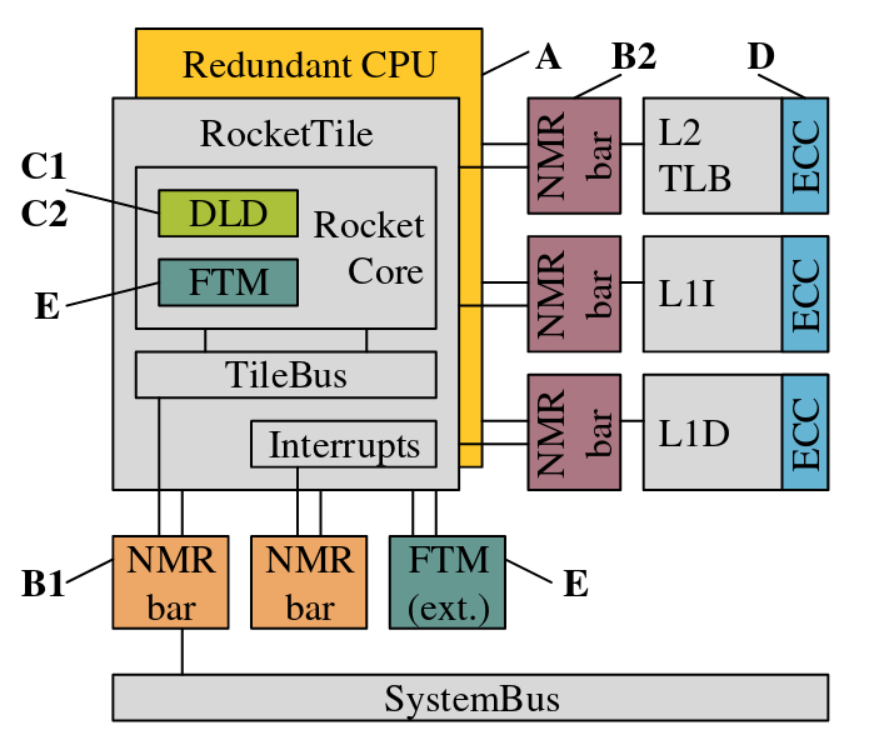
\includegraphics[width=0.45\textwidth]{framework_arch.png}
        \caption{Fault tolerant RISC-V framework's architecture}
        \label{framework_arch}
    \end{center}
\end{figure}

Authors in \cite{fault_tolerance_framework} have designed a framework to develop 
fault-tolerant solutions in such architecture. It is based on the Rocket 
processor \cite{rocket_chip_paper} and enables developers and
researchers to implement redundancy schemes easily due to the fact that the
different hardware-hardening techniques were written on \emph{Chisel} 
\cite{chisel_paper}, a high-level hardware design language that facilitates 
advanced circuit generation and design reuse for digital logic designs acting as 
a starting point for new developments.

The architecture of this framework implements several hardening-techniques
already, as depicted in Figure \ref{framework_arch}, it implements
\acrfull{NMRbar} to protect \acrfull{IO} from TileBuses, interrupts and memories
interfaces such as L1 and L2TLB caches; a redundant synchronized \acrfull{CPU} 
to implement a \acrshort{DCLS} technique; \acrfull{ECC} on memory caches for
error detection and correction; a \acrfull{DLD} that generates a fingerprint of
the internal registers on the \acrshort{CPU} enabling early detection of errors
before they propagate to other interfaces and, finally, an internal and external 
\acrfull{FTM} which resynchronizes the cores after an error occurrence,
indicates errors on its own \acrfull{CSR} and provide an external \acrfull{SPI}
interface which can be accessed externaly.

This architecture is fully and easily configurable, for instance the
\acrshort{NMRbar}s can be configured in a \acrfull{DMR} or a \acrshort{TMR} 
configuration, or the \acrshort{ECC} instances can be customized to select
different types of correction code (i.e. parity, \acrfull{SEC}, Hamming or, also
known as, \acrfull{SEC-DED}).

On another hand, although the default architecture of this framework already
provides a \acrshort{DCLS} scheme, it does not implements error-handling
and recovery techniques, which makes it suitable for the development of this
work as it provides an extension in the software-domain, making the framework
a \emph{hybrid} solution for future fault-tolerance projects.

\section{Scope and goals}

As a solution to the issues stated in Section \ref{soft_errors}, in this work is
proposed to develop a set of error-handling techniques within a \acrshort{DCLS}
with the following goals:

\begin{itemize}
    \item Analyze and study the state-of-the-art on error-handling techniques
        in software for fault-tolerance systems.
    \item Implement these techniques to recover the system to a healthy state on 
        the occurrence of a temporary soft-error.
    \item Maintain introduced overhead, in terms of size and time execution
        minimal, triggering these techniques in an intelligent manner.
    \item Extend the capabilities of the framework described in Section
        \ref{framework_riscv}, adding software error handling and recovery
        solutions for developers and researchers to implement easily.
\end{itemize}

The solution is implemented on a ZCU104 evaluation board, depicted in Figure
\ref{zcu104}, where the implementation is deployed and tested its correct
operation.

\begin{figure}[h!]
    \begin{center}
        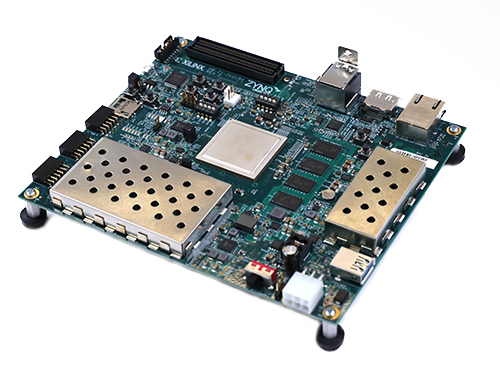
\includegraphics[width=0.7\textwidth]{zcu104.jpg}
        \caption{ZCU104 development board}
        \label{zcu104}
    \end{center}
\end{figure}


\chapter{Theoretical Background}
\thispagestyle{fancy}

This chapter describes the theoretical background of Lockstep technique and how
a \acrshort{DCLS} system is commonly implemented along state-of-the-art 
error-handling and recovery techniques in software.

\section{Lockstep}

Spacial modular redundancy techniques where first proposed on the early 1960s,
during the start of space programs since reliability provisions were required to
avoid human lives being at risk by computer failures in space. The initial
examples of lockstep proposals began in the early 2000s \cite{lockstep_patent},
by a pattent filed by \emph{Compaq Computer Corp.}

According to the autor in \cite{lockstep_analysis_thesis}, the term
\emph{lockstep} in the field of the embedded systems describes a mechanism to 
monitor and verify the correctness in the operation of a system by employing at 
least two \acrshort{CPU}s performing identical operations, and is part of the 
hybrid techniques domain presented in Chapter \ref{introduction}. 
Typically, the processors are synchronized to the same state during the system 
start-up. The same tasks are independently processed by the processors operating 
in lockstep and a real-time comparisson of the output signals is performed, 
where the output signal can be comparisson of the processor flags, registers or 
memory modules. Furthermore, in case of discrepancy in the output signals, an 
error signal is generated and further execution of the task is inhibited, 
leading to a faulty state of the system, which must be handled by the system
developer and is dependent upon the architecture in question. A high-level block 
diagram of this methodology extended to a Dual Core architecture is depicted 
Figure \ref{lockstep_diagram}. The main benefit of this method is its simplicity
and has been extensively implemented by semiconductors companies, for example
the ARM Cortex-R5 implements a dual-core processor which can be configurated for
either a redundant CPU in lock-step for fault tolerant/fault detecting
dependable systems or dual cores running independently, each executing its own
program with its own bus interfaces, interrupts and so on.

\begin{figure}[h!]
    \begin{center}
        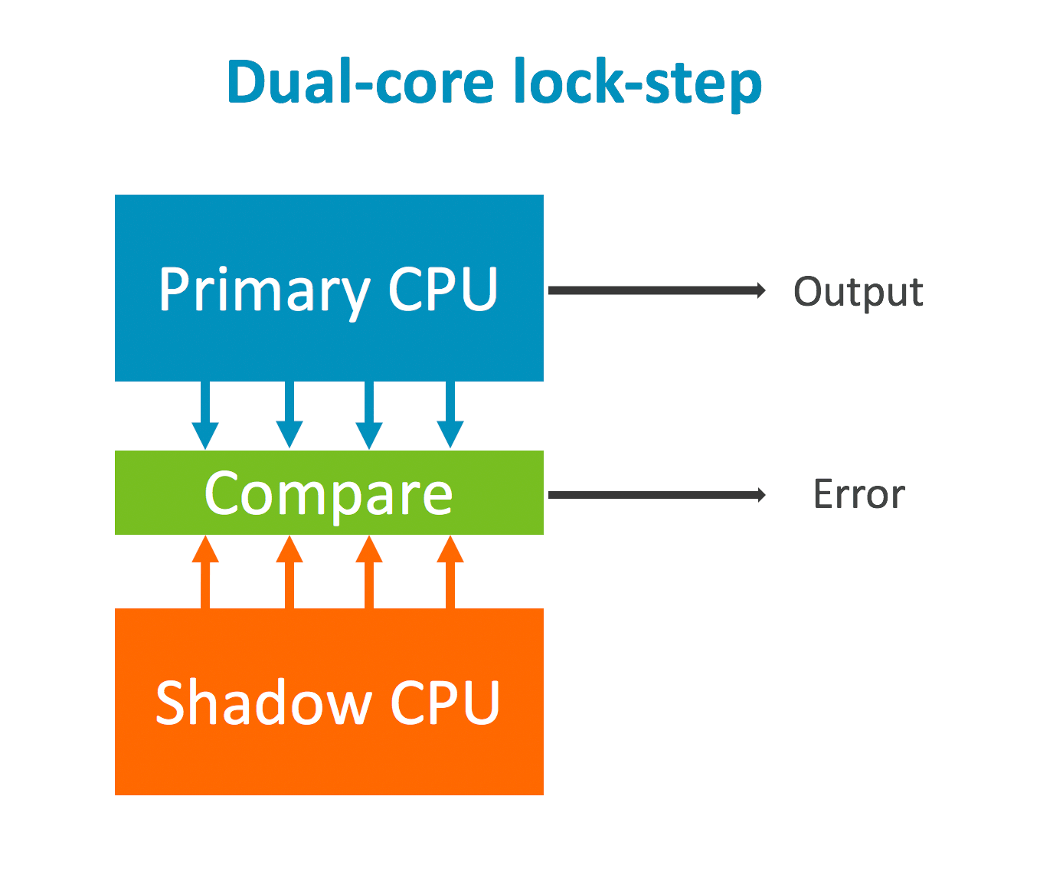
\includegraphics[width=0.4\textwidth]{lockstep_diagram.png}
        \caption{High-level block diagram of a Dual Core Lockstep mechanism}
        \label{lockstep_diagram}
    \end{center}
\end{figure}

The lockstep technique's most significant benefit is its ability to detect both
\acrshort{SDC}s and \acrshort{FI}s, in contrast to many other fault tolerance
techniques, but on its own is not capable of correcting and recovering from such
situations, that is the main reason why Lockstep techniques in hardware are
coupled with error handling and recovery software, making it a hybrid
fault-tolerance solution. There are several software techniques for such goals
that are described in the following Sections.

\section{Re-execution}

As mentioned previously, after a transient fault is detected by the lockstep
mechanism, a fault tolerance mechanism has to be invoked to handle such
situation. The simplest fault tolerance technique available in the current
literature \cite{reexecution_paper} is re-execution. With re-execution, a
process is executed again if affected by faults. 

Although its simplicity, when a process is re-executed after a fault has been
detected, the system restores all initial inputs of that process to the initial
state of the application running. This process requires time for its recovery,
denoted as \emph{recovery overhead}. Furthermore, all the progress of the
application has been lost, and for comparisson purposes, this will be counted as
overhead of the methodology.

\section{Rollback Recovery with Checkpointing}

The time needed for re-execution can be substantially reduced with more complex
fault tolerance techniques such as \emph{rollback recovery with checkpointing}.
The main principle of this technique is to restore the last non-faulty state of
the failing process. The last non-faulty state, also known as \emph{checkpoint},
has to be saved in advance in the static memory and will be restored if the
process fails, this method takes for granted that the memory in which
this \emph{checkpoint} is stored it is hardened against soft-errors. The part of
the process between two checkpoints or between a checkpoint and then of the
process is caled an \emph{execution segment}, this implies that the
\emph{re-execution} mechanism is a \emph{Rollback recovery} with only one
checkpoint, which is the starting point of the application.

Checkpoints must be stored during the whole execution of the application, this
can be done in an intelligent manner, where saving of the process states is the
fastest. However, this approach is \emph{application-specific} requiring prior
knowdlege of application details. On another hand, \emph{checkpointing} can be
done \emph{systematically}, for example, at equal intervals.

Authors in \ref{rollforward_error_recovery} have depicted an example of this 
mechanism, which can be seen in Figure \ref{rollback_diagram}, here two parallel 
systems are executing the same application, $\mathrm{T_{ch}}$ is the time 
required to create and store the checkpoint, $\mathrm{t_{cp}}$ is the time 
required to make the state of the modules consistent with the state saved in one 
of the modules, in this case, checkpointing is done periodically, where the 
interval is denoted by $\mathrm{I_j}$, and, finally, $\mathrm{t_r}$ is the time 
required to make the rollback.

\begin{figure}[h!]
    \begin{center}
        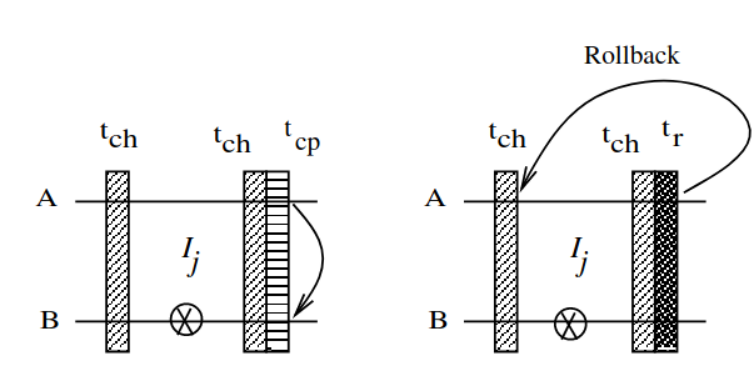
\includegraphics[width=0.7\textwidth]{rollback_diagram.png}
        \caption{Rollback in duplex systems timeline.}
        \label{rollback_diagram}
    \end{center}
\end{figure}

\section{Rollforward recovery with checkpointing}

Once again, as happened with re-execution, rollback also adds some overhead
execution by retrying an \emph{execution-segment} that was already executed
before. In order to avoid this overhead in time-execution, authors in
\cite{rollforward_error_recovery} have proposed a rollforward technique. This
technique is based on a spare processor, which when a checkpoint mismatch
occurs, during the validation step, the two processors continue execution while
the spare processor retries the task to determine which of the diverged
processors is fault-free, once the faulty processor is detected, the application
continues while the state of the faulty processor is replaced by a healthy-state
to continue its operation. This roll-forward checkpointing scheme is depicted in
Figure \ref{rollforward_scheme}, there can be seen the Spare processor running
the \emph{faulty} checkpoint and verify which of the two main processors is
failing.

\begin{figure}[h!]
    \begin{center}
        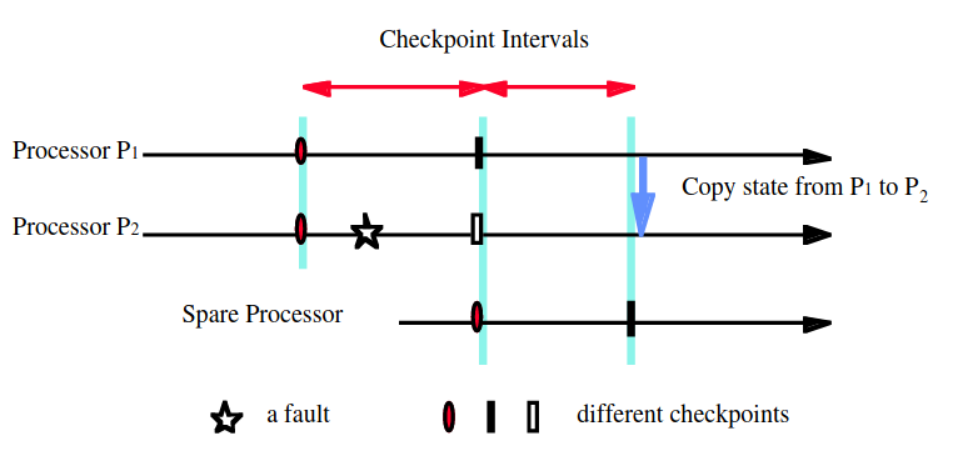
\includegraphics[width=0.5\textwidth]{rollforward_scheme.png}
        \caption{Roll-forward checkpointing scheme}
        \label{rollforward_scheme}
    \end{center}
\end{figure}

The major advantage of this scheme is that it has lower overhead of the recovery
action, with the cost of a spare processor and the fact that this scheme must
retain any result that is to be delivered to an external environment, such as
other task or peripherals. Which could be still a significant drawback for a
time-critical applications if the deadline is not met.

Furthermoure, although this scheme avoids the use of a rollback mechanism, if
this task fails on the last two checkpoints, it is necessary to apply the latter
on order to restore the system to a healthy state.

Finally, during the validation step, if the three processor missmatch, then the
system should restore the two main processors to a known healthy checkpoint, or
even so restart the whole system.

\chapter{Implementation}
\thispagestyle{fancy}

\chapter{Benchmarking and results}
\thispagestyle{fancy}

\chapter{Conclusions}
\thispagestyle{fancy}

\begin{printbibliography}
    \thispagestyle{fancy}
\end{printbibliography}

% Print table of acronyms
\begin{printnoidxglossaries}
    \thispagestyle{fancy}
\end{printnoidxglossaries}

\end{document}
